The calorimeter high-level trigger (HLTCalo) is used to trigger on physics objects that deposit their energy in either the electromagnetic or hadronic calorimeter.
As described in Section \ref{sec:Det:Calo} the calorimeter is segmented into cells.
These cells are clustered together, as described in Section \ref{sec:Det:Calo} , and can be combined with inner detector tracks, to define physics objects such as electrons, photons, taus, and jets. 

The HLTCalo is monitored to check the performance and consistency of the triggers. 
This is achieved by monitoring the individual cells in the calorimeters and also comparing the different L2 and EF triggered physics objects to the corresponding offline object.
Monitoring flags are defined for each monitoring distribution, where a green flag represents the distribution is consistent with the expected distribution, and yellow and red represent a deviation from the expected distribution. 
When the flag is red or yellow the distribution is studied further to find the reason, and if necessary can then be excluded from physics analysis.


In this chapter, work done by the author on improvements to the current cell monitoring which expose hot cells, and the addition of monitoring of calorimeter objects are discussed. 

\section{Cells}

To monitor the overall HLTCalo, monitoring is done on the cells of the calorimeter.
This monitoring consists of distributions showing the number of active cells in the LAr and Tile, the number of problematic cells and the position of these cells in the LAr and Tile, and also the difference in cell energy between the trigger levels and offline levels.

The number of cells in the LAr and Tile is an example of a monitoring plot that is very stable and  should only change when a hot cell is masked or taken offline, allowing very tight flag definitions.
Monitoring plots, such as the percentage difference in energy in the trigger and offline cells, vary significantly ($\sim15\%$) with different running conditions, so either looser or no flag definitions are set.

The average transverse energy per cell in $\eta  \phi$ distribution is important in identifying hot spots where one cell records artificially high energy in every event.
Hot cells can be caused from electronics problems within the cells. 
Figure \ref{SW_hotspot} shows an example of a hot spot found using the offline cell monitoring in run 201191, resulting in the cell being masked (***Check with Denis****).

\begin{figure}
\centering
\mbox{
   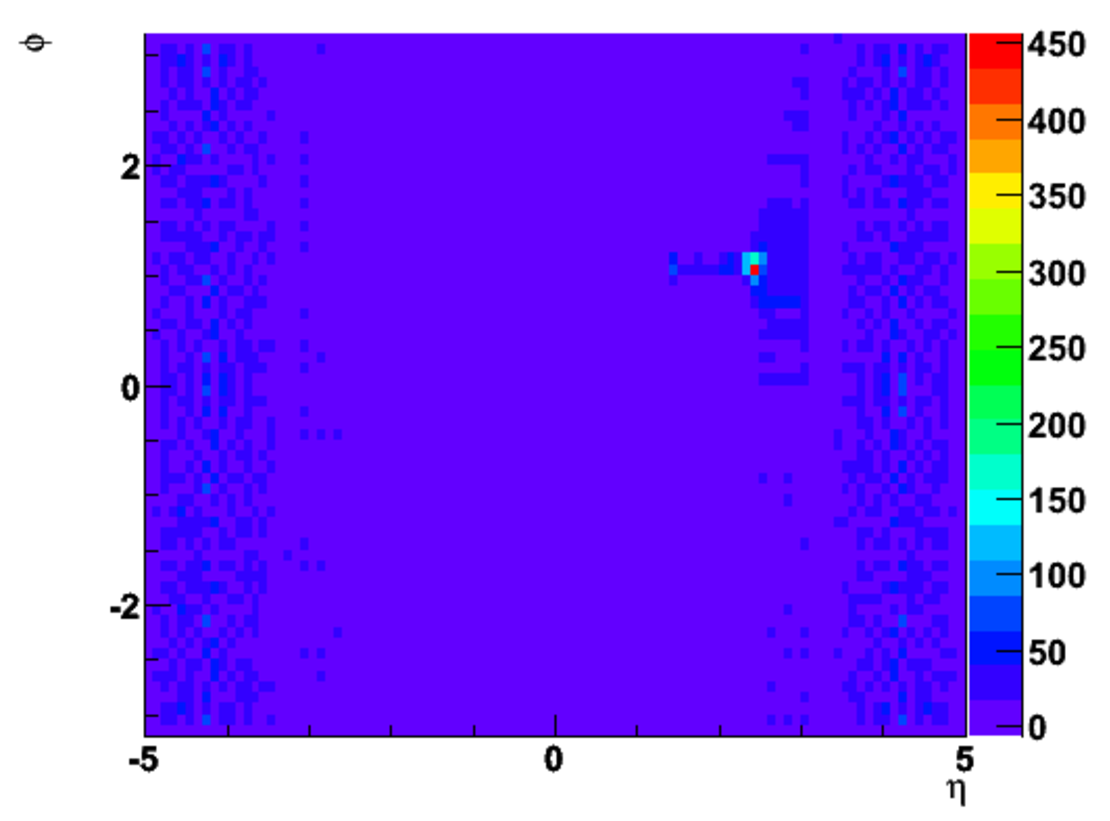
\includegraphics[width=0.9\textwidth]{figures/ServiceWork/Cells_HotSpot.pdf}
}
\caption[Offline egamma \et{} verses L2/EF egamma \et{}]{Average \et{} per $\eta \phi$ bin in run 201191. A clear hot region is observed at $\eta=2.5$ $\phi=1$. \label{SW_hotspot}}
\end{figure}



\section{Calorimeter Objects}

The HLTCalo is also monitored by comparing calorimeter triggered objects (electrons, photons and jets) and to the offline objects.
A cut on the \dr{} is done to match the triggered objects to the offline objects.
An \et{} cut has been applied to the offline objects, which is consistent with the analysis cut required when using the object. 



\subsection{Electrons and Photons}



%-Define the offline and two trigger clusters
%-explain difference between two trigger level clusters
%-Show the matching cuts
%-Explain the reason for the plots
%-For the plot, make sure we explain the red points.

The EM calorimeter component of the HLTCalo is monitored by using physics objects that are reconstructed using EM energy deposits from electrons and photons. 
There are differences between the L2 and EF level EM cluster finding due to the time constraints on the L2 trigger.  
The L2 EM clusters are found using only the second EM calorimeter layer, in which the highest energy cell is used as the cluster seed.
From this cluster seed, the cluster position is formed using the energy weighted $\eta$ $\phi$ from a grid of \etaphiB{0.075} around the seed, and the cluster energy is calculated by summing over the energy of the cells. 
Conversely, the EF EM clusters use a sliding-window cluster algorithm using the calorimeter towers. 
This reduces the effect of the hot cells, as these will be smeared by the surrounding regular cells which will not have energy deposits.
The offline clusters are also found using a sliding-window algorithm, but they have full offline cell information.
 

\subsubsection{EM cluster matching}

Matching the offline and trigger objects is done using \dr{}.
Figure \ref{SW_egamma_L2_dR} shows the \dr{} distribution between the offline and all L2 EM clusters.
Two peaks can be seen in (a), one at $\dr{}=0$ which corresponds to good matching.
Events often have two objects that will be back-to-back in \dphi{}, which corresponds to the peak at $\dr{}\approx\pi$. 
The peak at $\dr{}=0$ shown in the expanded view (b), which shows a minimum in the range \dr{} from 0.03 to 0.1.

Figure \ref{SW_egamma_EF_dR} shows the \dr{} distribution between the offline and all EF EM clusters.
As observed for the L2 \dr{} distribution, there are two peaks; one at $\dr{}=0$ and one at $\dr{}\approx\pi$. 
The minimum observed in (b) is in the range \dr{} from 0.02 to 0.1.

A \dr{} matching cut of 0.035 is used between the offline and both L2 and EF triggers as this selects the majority of the correctly matched clusters and is also the distance from the centre to the edge of the L2 cluster.
In addition, the offline cluster is required to have $\et{}>10$ GeV.  

\begin{figure}
\centering
        \begin{subfigure}[b]{0.5\textwidth}
                \centering
                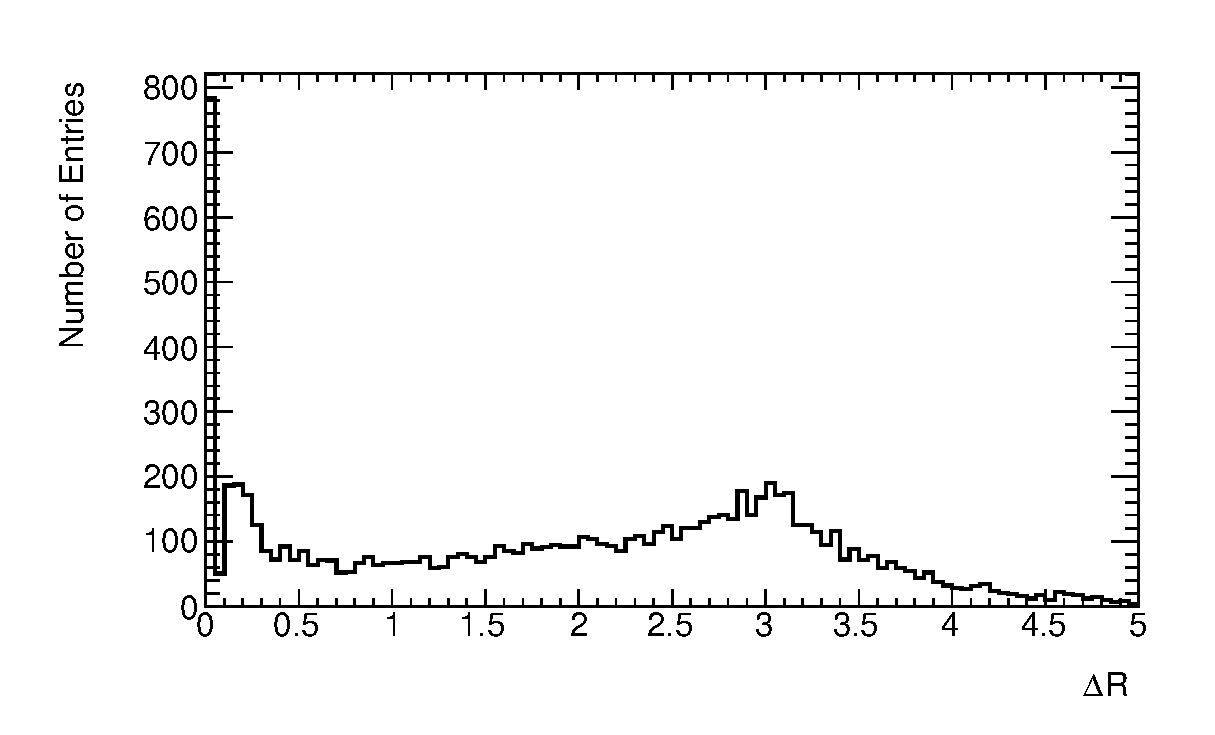
\includegraphics[width=\textwidth]{figures/ServiceWork/EgammaL2/DR_Unmatched_L2.eps}
        \end{subfigure}%
        \begin{subfigure}[b]{0.5\textwidth}
                \centering
                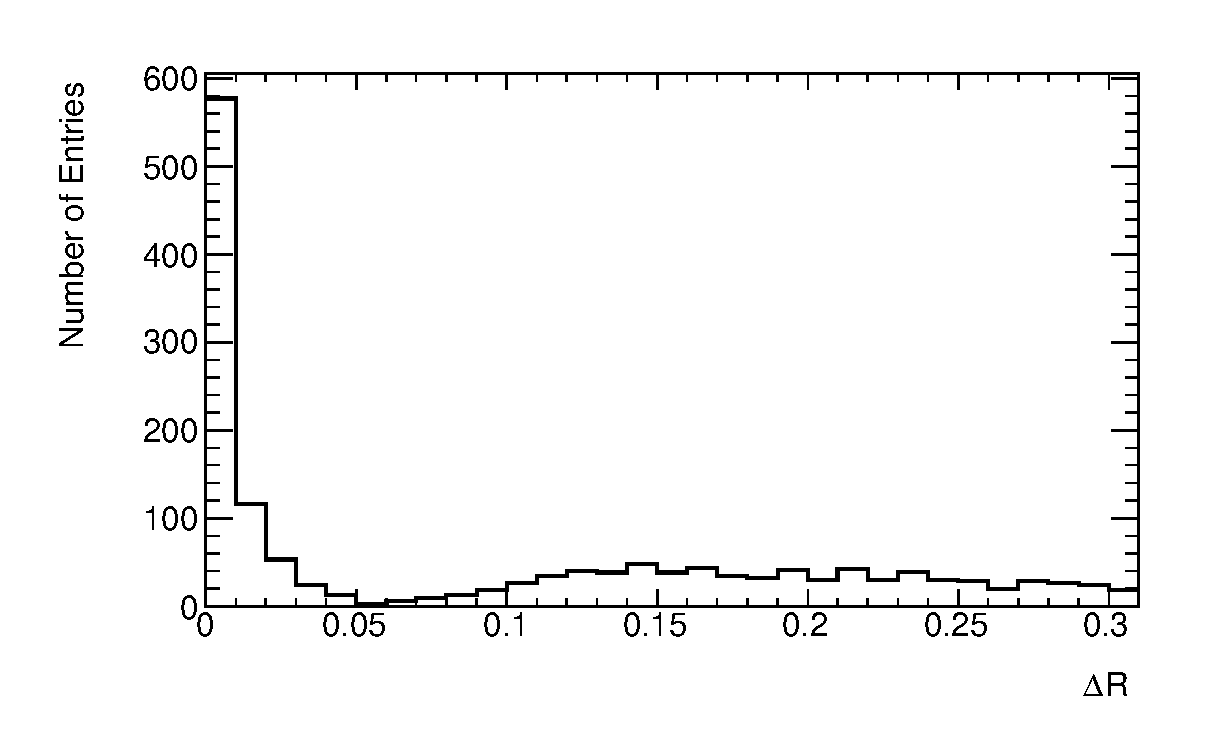
\includegraphics[width=\textwidth]{figures/ServiceWork/EgammaL2/DR_Unmatched_Zoomed_L2.eps}
        \end{subfigure}%
\caption[\dr{} between offline and L2 EM object]{
\dr{} distribution between the offline EM cluster and all L2 clusters in the event, shown within the range (a) $0 - 5$ and (b) $0 - 0.3$. 
\label{SW_egamma_L2_dR}}
\medskip
        \begin{subfigure}[b]{0.5\textwidth}
                \centering
                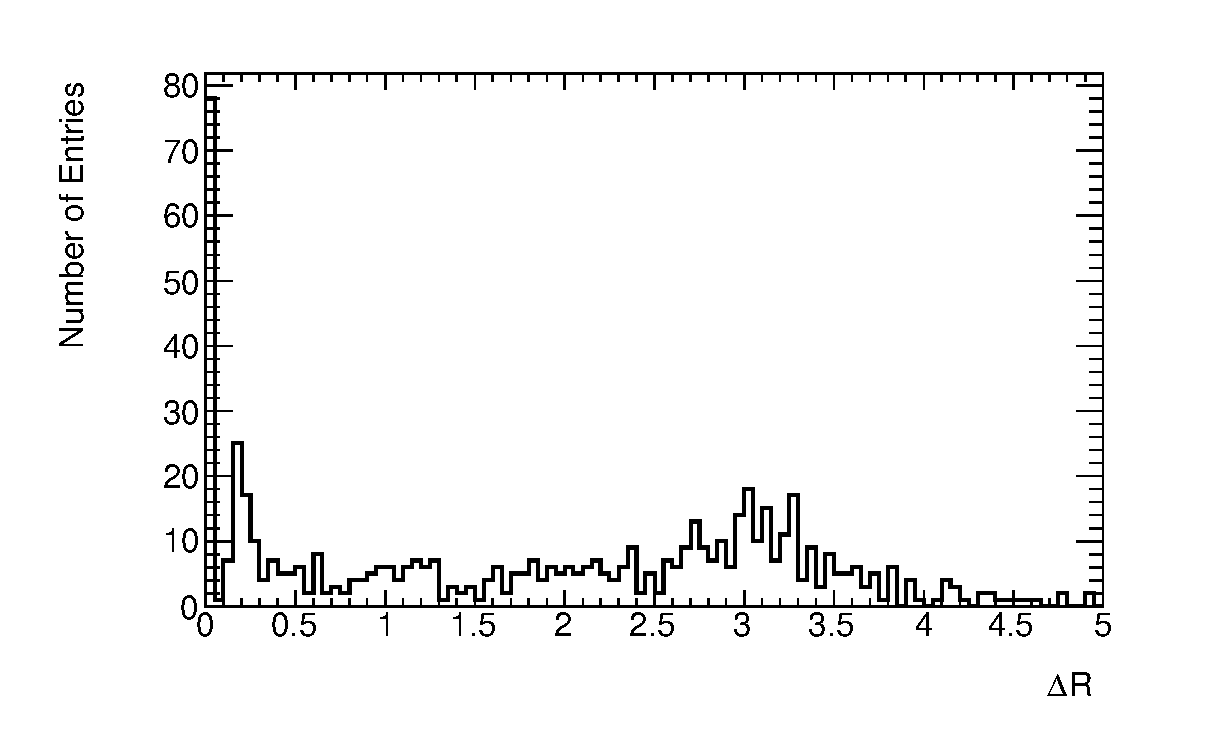
\includegraphics[width=\textwidth]{figures/ServiceWork/EgammaEF/DR_Unmatched_EF.eps}
        \end{subfigure}%
        \begin{subfigure}[b]{0.5\textwidth}
                \centering
                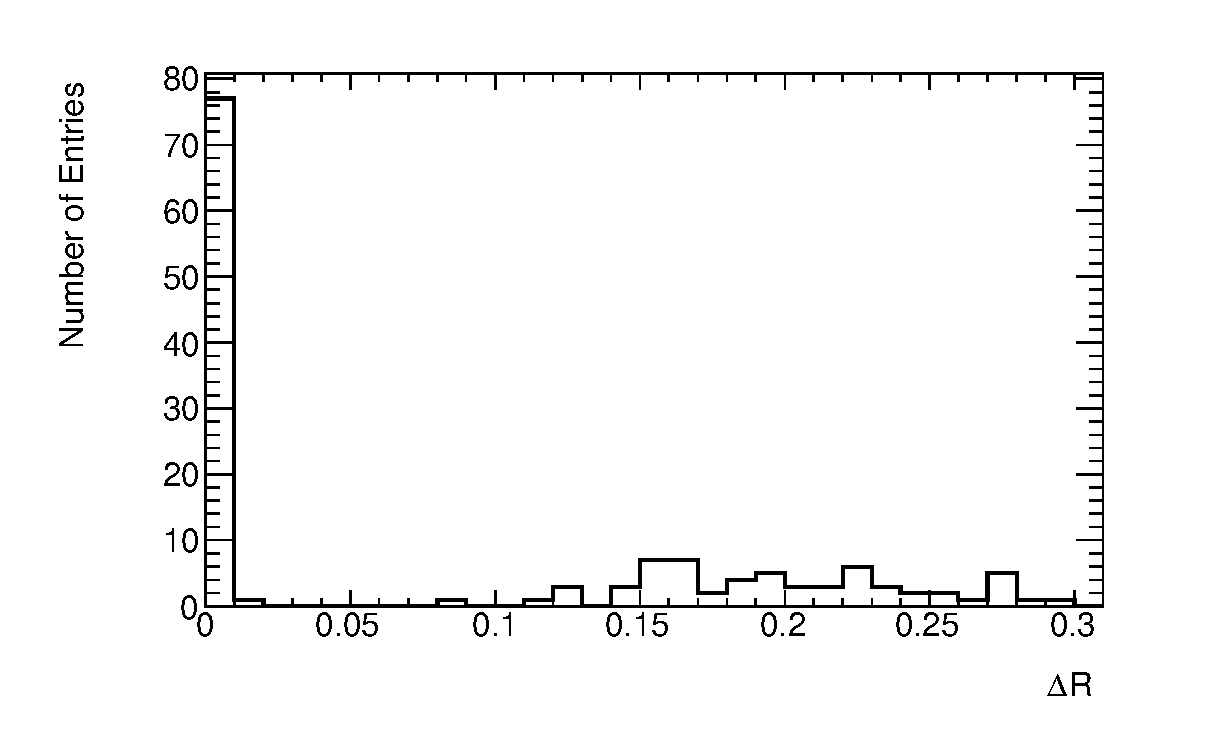
\includegraphics[width=\textwidth]{figures/ServiceWork/EgammaEF/DR_Unmatched_Zoomed_EF.eps}
        \end{subfigure}%
\caption[\dr{} between offline and EF EM object]{
\dr{} distribution between the offline EM cluster and all EF clusters in the event, shown within the range (a) $0 - 5$ and (b) $0 - 0.3$. 
\label{SW_egamma_EF_dR}}
\end{figure}




\subsubsection{Monitored Distributions}


The monitoring plots shown in Figures \ref{SW_egamma_L2EF_EtEt} -\ref{SW_egamma_L2EF_Reso} are from run 190644 in the  2011 data-taking.
Figure \ref{SW_egamma_L2EF_EtEt} shows the distribution of the offline EM cluster \et{} versus that of (a) a L2 and (b) a EF EM cluster \et{}.
This is useful in checking the linearity of the trigger EM clusters to the offline. 
The L2 EM cluster \et{} shows good linearity to the offline EM cluster \et{}, and the majority of events fall on a straight line where the \et{} of the offline and L2 are the same.
There is a significant band either side of this straight line, with more falling above the line.
This corresponds to a larger offline \et{} than L2 EM cluster \et{}.
The EF EM cluster \et{} has an even better linearity, and again most of events fall on a straight line corresponding to the offline EF clusters having the same \et{}.
The band around the events falling on the straight line is significantly smaller than for the L2 EM clusters.


Figure \ref{SW_egamma_L2EF_EtFrac} shows the distribution of \et{} fraction,
\begin{equation}
f(\et{})_{Trigger}=\frac{\et{}(\rm{Triggered~EM~cluster})}{\et{}(\rm{Offline~EM~cluster})},
\label{SW:EtFrac}
\end{equation}
as a function of $\eta{}$ for (a) the L2 EM clusters and (b) the EF EM clusters.
The \et{} fraction for the L2 EM clusters is centred around one, with most events within $5\%$.
The EF EM clusters' \et{} fraction is also centred around one, but with significantly smaller fluctuations.
In both distributions there is a region at $|\eta{}|=1.5$ where the fluctuations in the ratio from unity are larger.
This is due to the EM deposit falling into the crack region between the EM calorimeter barrel and the EM barrel end-cap.
There is an improvement in the EF due to the additional calibration done at EF level. 

Figure \ref{SW_egamma_L2EF_Reso} shows the distribution of the \et{} resolution,
\begin{equation}
\sigma(\et{}) =\frac{\et{}(\rm{Triggered~EM~cluster})-\et{}(\rm{Offline~EM~cluster})}{\et{}(\rm{Offline~EM~cluster})},
\label{SW:EtReso}
\end{equation}
for (a) L2 EM clusters and (b) EF EM clusters.
Both distributions have a mean $\sigma(\et{})$ of $<1\%$. 
The L2 EM cluster $\sigma(\et{})$ distribution has a larger spread than that for the EF.


All the monitoring distributions are susceptible to changes in calibration or the cluster sizes. 
The monitoring flags can be set to compare the mean of the distribution to the expected value.
The distributions in Figures \ref{SW_egamma_L2EF_EtFrac} and \ref{SW_egamma_L2EF_Reso} have flags set based on the mean of the \et{} fraction and $\sigma(\et{})$, respectively. 
If these show sizable differences from the expected mean, the distribution will be yellow or red flagged automatically.
Figure \ref{SW_egamma_L2EF_EtEt} can then be used to study the reason for the differences.

 
\begin{figure}
\centering
        \begin{subfigure}[b]{0.5\textwidth}
                \centering
                \includegraphics[width=\textwidth]{figures/ServiceWork/run_190644/EtEt_Matched_L2.eps}
        \end{subfigure}%
        \begin{subfigure}[b]{0.5\textwidth}
                \centering
                \includegraphics[width=\textwidth]{figures/ServiceWork/run_190644/EtEt_Matched_EF.eps}
        \end{subfigure}%
\caption[Offline EM \et{} versus L2 and EF EM \et{}]{
\et{} of the offline EM cluster versus the \et{} of the closest matched (a) L2 and (b) EF EM cluster.
\label{SW_egamma_L2EF_EtEt}}
\end{figure}

\begin{figure}
\centering
        \begin{subfigure}[b]{0.5\textwidth}
                \centering
                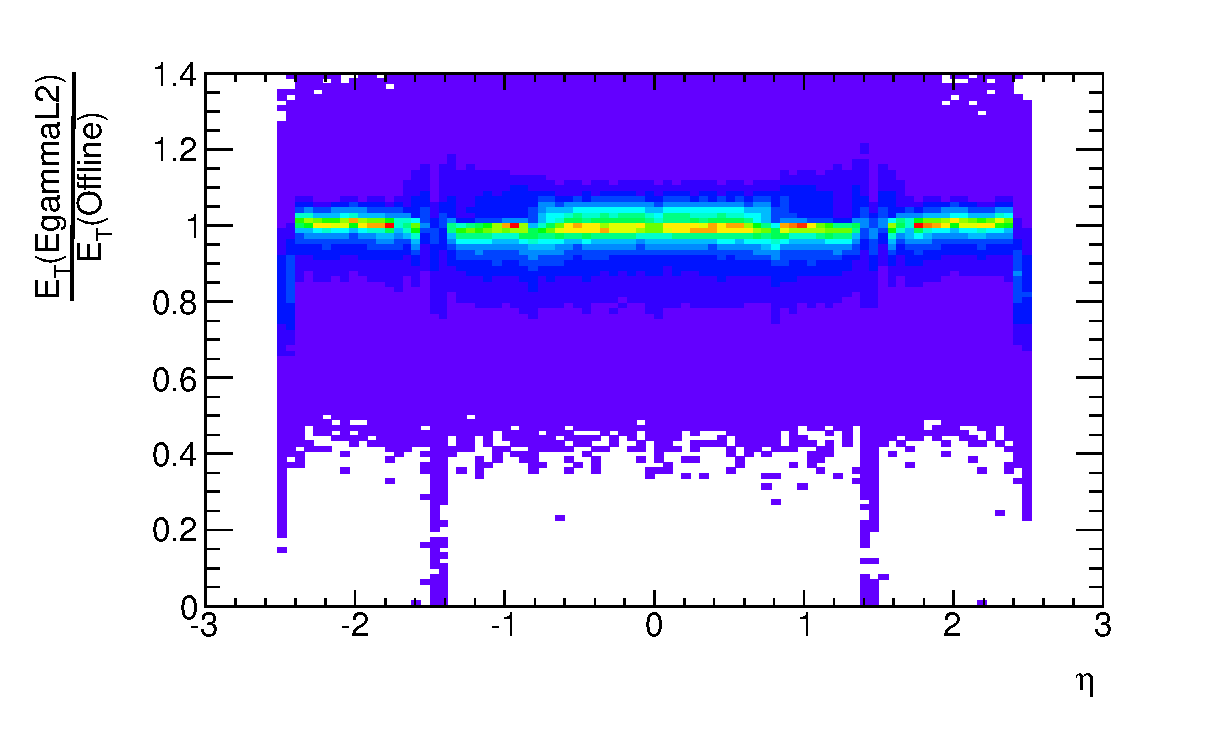
\includegraphics[width=\textwidth]{figures/ServiceWork/run_190644/EtFrac_Eta_Matched_L2.eps}
        \end{subfigure}%
        \begin{subfigure}[b]{0.5\textwidth}
                \centering
                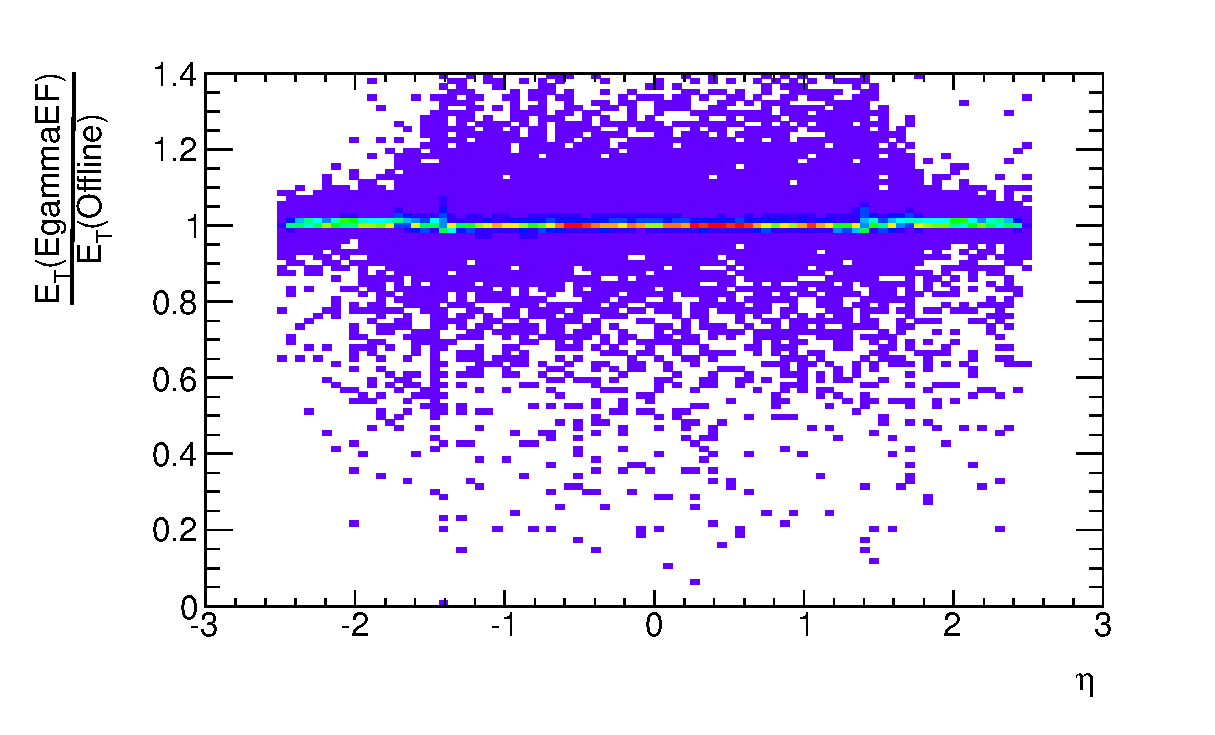
\includegraphics[width=\textwidth]{figures/ServiceWork/run_190644/EtFrac_Eta_Matched_EF.eps}
        \end{subfigure}%
\caption[\et{} fraction of L2 and EF to offline EM objects]{
\et{} fraction of (a) the  L2 and (b) the EF EM cluster  to the offline EM cluster \et{} as a function of $\eta$. 
\label{SW_egamma_L2EF_EtFrac}}
\end{figure}

\begin{figure}
\centering
        \begin{subfigure}[b]{0.5\textwidth}
                \centering
                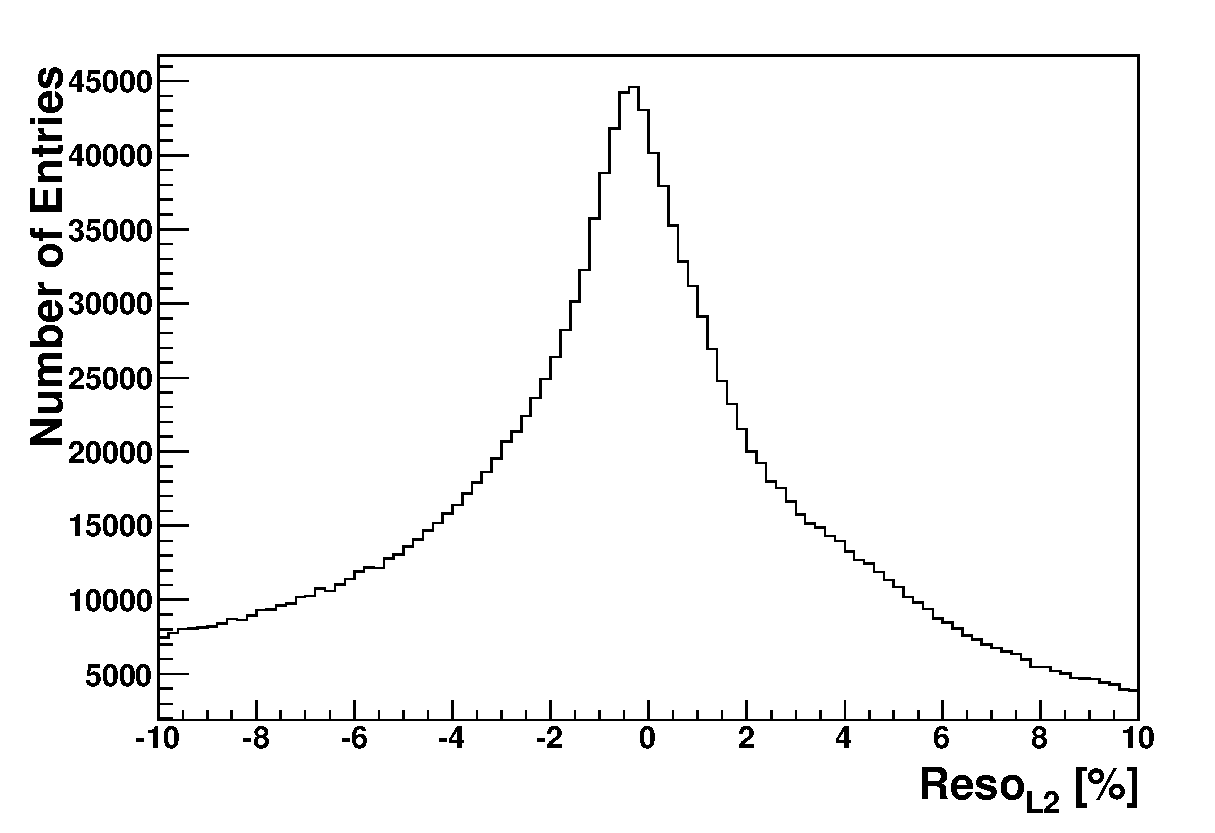
\includegraphics[width=\textwidth]{figures/ServiceWork/run_190644/Reso_Matched_L2.eps}
        \end{subfigure}%
        \begin{subfigure}[b]{0.5\textwidth}
                \centering
                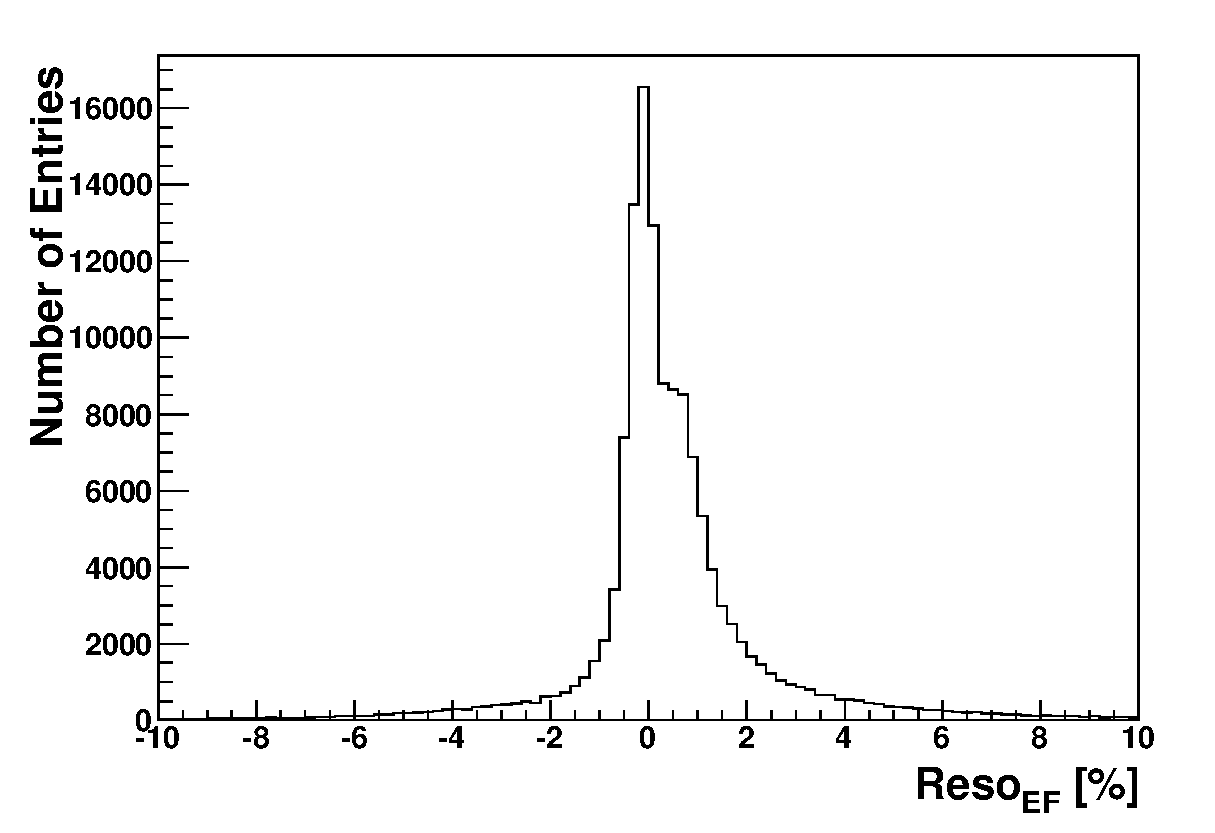
\includegraphics[width=\textwidth]{figures/ServiceWork/run_190644/Reso_Matched_EF.eps}
        \end{subfigure}%
\caption[Offline EM \et{} versus L2/EF EM \et{}]{
Distribution of the relative difference between the \et{} of the (a) L2 and (b) EF EM cluster, and the offline EM cluster \et{}.
\label{SW_egamma_L2EF_Reso}}
\end{figure}


Figure \ref{SW_egamma_EF_Reso_Range} shows the history of the mean of $\sigma(\et{})$ for EF EM clusters.
The colours of the points show the flag that was set for these runs.
Flags were assigned for a given run depending on the difference of the mean to a standard mean of $0.975\%$. 
The run is flagged green if the difference is less than $0.2\%$, yellow if between $0.2\% - 0.4\%$ or red if greater than $0.4\%$.
These flag values were tuned using the initial runs in the first data taking region.
Most of the runs are set as green or yellow, with only a few set as red.
The red flagged runs are those where there is no stable beam and some sections of the LAr calorimeter were not online during the run.


\begin{figure}
\centering
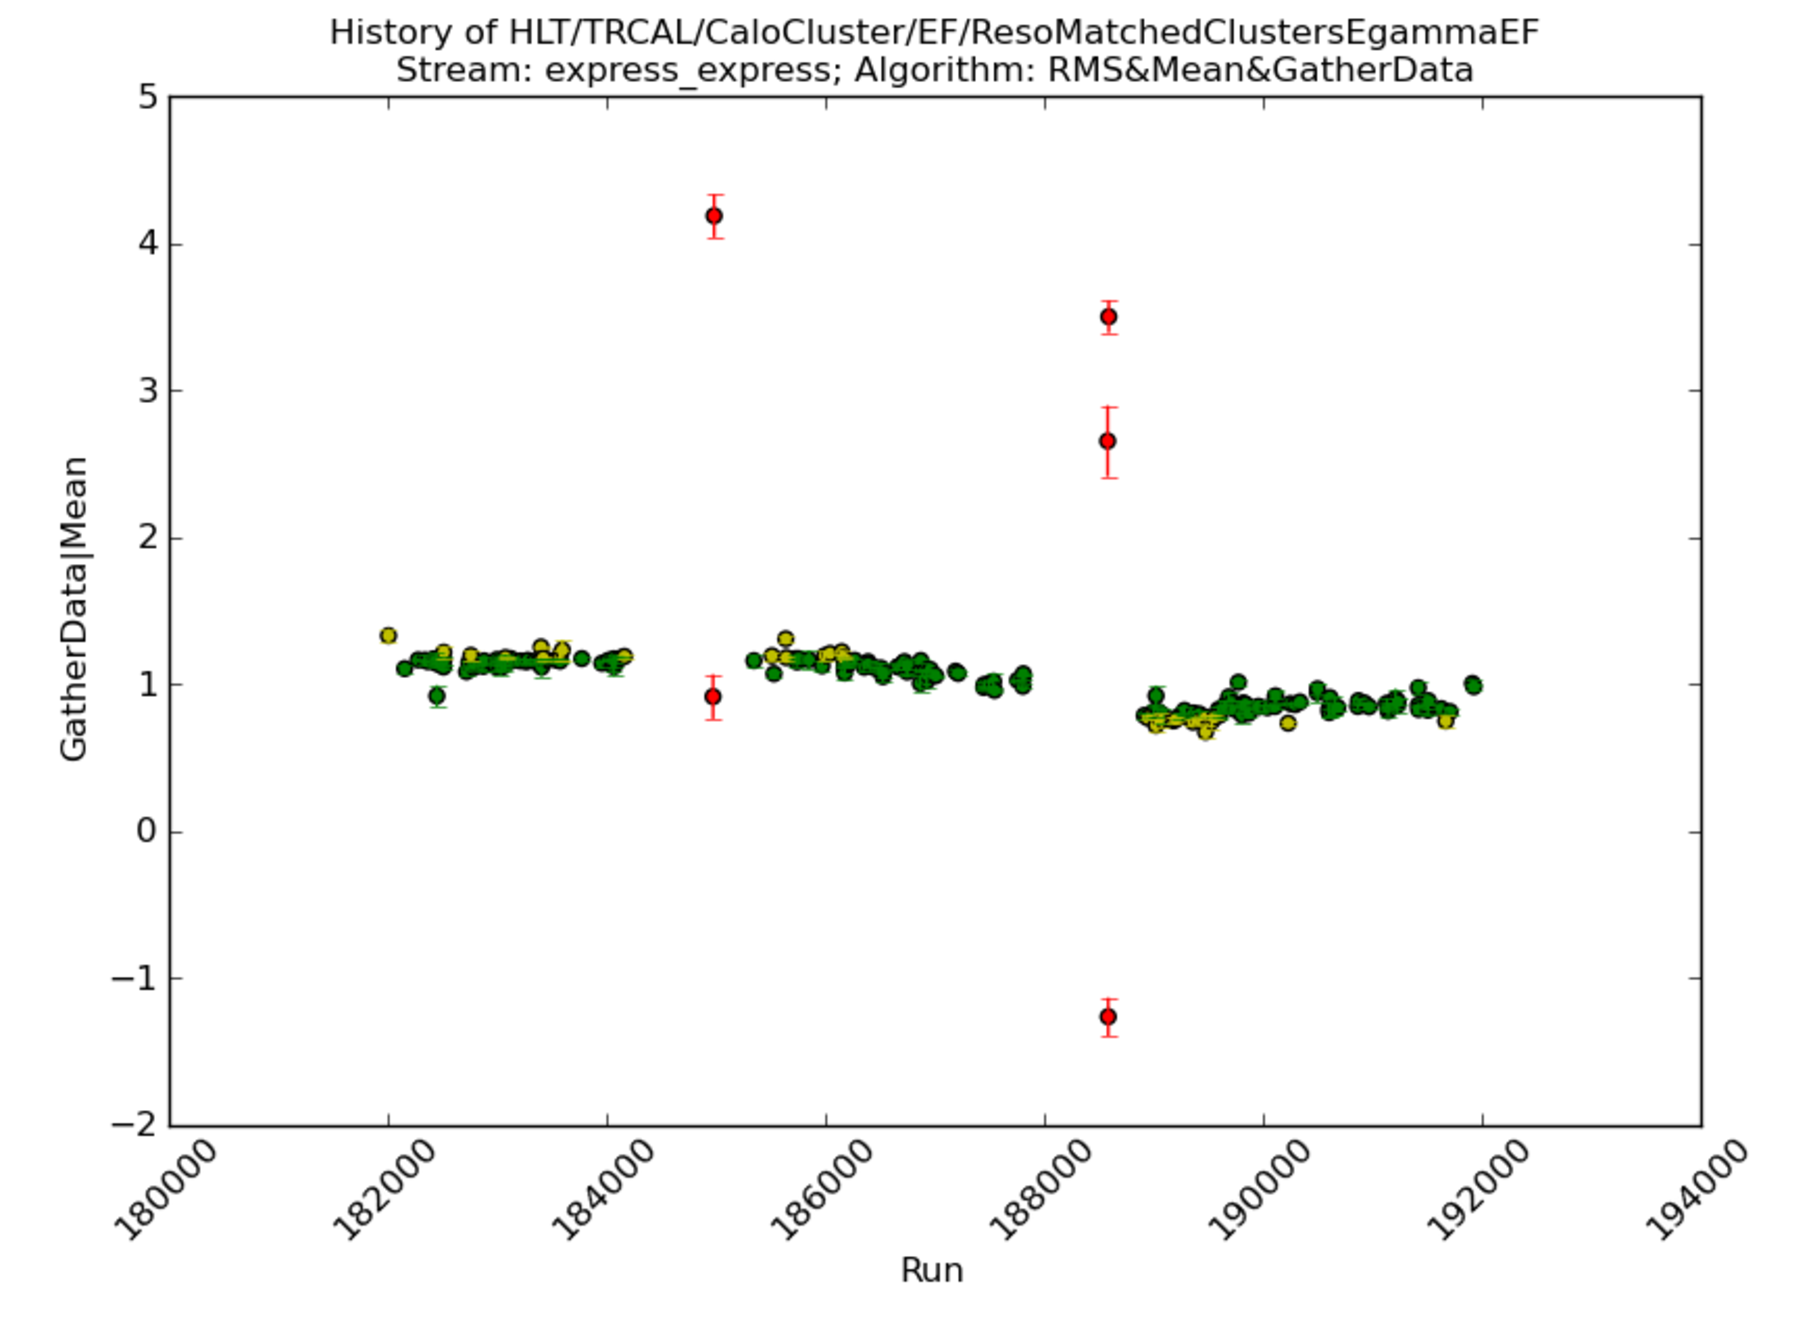
\includegraphics[width=1.0\textwidth]{figures/ServiceWork/EF_Reso_Range.pdf}
\caption[Mean EF EM cluster \et{} resolution as a function of run number]{
Mean EF EM cluster $\sigma(\et{})$ as a function of run number. 
\label{SW_egamma_EF_Reso_Range}}
\end{figure}


 
\subsection{Jets}
\label{HLTCalo:Jets}

%-Define the offline and two trigger jets 
%-need to explain what we really want to show.
%-Show the matching cuts
%-Explain the reason for the plots
%-For the plot, make sure we explain the red points.

Studying triggered and offline EM clusters monitors the EM calorimeter. 
Jets are used to study the hadronic calorimeter.
These jets consist of grouping of EM and hadronic clusters.

The \antikt{} jet-finding algorithm, which is described in Section \ref{sec:Theory:Jets}, was used with an R parameter of 0.4 for the offline jets.
The minimum \pt{} cut applied on the offline jets corresponds to the standard analysis cut of 20 GeV.


The L2 jet-finding is done using a cone algorithm.
The cone algorithm is seeded using a L1 RoI, and all deposits within the radius of the cone are combined, and a new cone centre is defined using the energy weighted position of the constituents.
With the new cone defined, any new deposits within the radius are again combined, and a new cone centre is defined.
This continues until the cone centre does not change.

The \antikt{} jet-finding algorithm is used for the EF jets. 
While it is the same jet-finding algorithm, the EF jets run over clusters that are close to the RoI.

In the 2012 data taking, calibration is applied to the EF jets to account for the non-compensating calorimeters. 

\subsubsection{Jet matching}

The trigger jets are matched to offline jets to allow them to be compared.
This matching is achieved by applying a \dr{} cut.
Figure \ref{SW_jet_L2_dR} shows the \dr{} between the offline jets and all L2 jets in the event.
As observed in the EM clusters, in (a) there are two peaks; one at $\dr{}\approx0$ and one at $\dr{}\approx3$.
The differences from the EM clusters are best seen in (b), the first peak is not quite at zero.
This is due to the $\phi$ resolution of the jets moving the \dphi{} away from zero. 
Figure \ref{SW_jet_EF_dR} shows the \dr{} between the offline jets and all EF jets in the event.
The distributions are similar to the L2 jet \dr{} distributions, with a peak just above zero, and one at $\dr{}\approx3$. 

A \dr{} matching cut of 0.4 is used for both the L2 and EF jets.
This value corresponds to the R value used in the jet-finding for both the trigger and offline jets.

\begin{figure}
\centering
\mbox{
              \subfigure[]{\epsfig{figure=figures/ServiceWork/Jets/L2_DRUnmatchedJetsJet.eps,width=0.5\textwidth}}\quad
              \subfigure[]{\epsfig{figure=figures/ServiceWork/Jets/L2_DRUnmatchedJetsZoomedJet.eps,width=0.5\textwidth}}\quad
                              }
\caption[\dr{} between offline and L2 jets]{\dr{} between the offline jet and all L2 jets in the event, shown with range (a) $0 - 6$ and (b) $0 - 1$ \label{SW_jet_L2_dR}}
\end{figure}

\begin{figure}
\centering
\mbox{
              \subfigure[]{\epsfig{figure=figures/ServiceWork/Jets/EF_DRUnmatchedJetsJet.eps,width=0.5\textwidth}}\quad
              \subfigure[]{\epsfig{figure=figures/ServiceWork/Jets/EF_DRUnmatchedJetsZoomedJet.eps,width=0.5\textwidth}}\quad
                              }
\caption[\dr{} between offline and EF jets]{\dr{} between the offline jet and all EF jets in the event, shown with range (a) $0 - 6$ and (b) $0 - 1$ \label{SW_jet_EF_dR}}
\end{figure}



\subsubsection{Monitored Distributions}

The jet monitoring uses the same distributions as the monitoring of the EM clusters.
The monitoring distributions shown in Figures \ref{SW_jet_L2EF_EtEt} - \ref{SW_jet_L2EF_Reco} are from run 203335, which was taken in 2012.

Figure \ref{SW_jet_L2EF_EtEt} shows the \et{} of the offline jet versus (a) the L2 and (b) the EF jets.
The \et{} comparison is used to check the linearity of the trigger jet \et{} to that of the offline jet.
The L2 trigger \et{} shows linearity to the offline jet \et{}, with the trigger jets \et{} being $\approx 60 \%$ of the offline jet \et{}. 
This is due to the different energy scales of the jets; whilst the offline are fully calibrated, the L2 trigger jets are at EM scale.
The \et{} of the EF jets agree well with the offline jets. 
This improvement is expected due to the calibration done on the EF jets.
Both the EF jets and the L2 jets have good linearity to the offline jet \et{}.

Figure \ref{SW_jet_L2EF_EtFrac_Eta} shows the \et{} fraction as a function of jet $\eta$ for (a) the L2 jets and (b) the EF jets.
The L2 jets have a mean \et{} fraction of $\approx 0.7$, whilst the EF jets have a mean \et{} fraction closer to one.  
This is again explained due to the jet energy scale of the trigger jets.
In both distributions, underlying differences between the trigger jets and offline jets can be seen in different regions of the detector.
The jumps in $f(\et{})$ at $|\eta|\sim1.2$ are due to the transition between the barrel and the tile calorimeters, and large fluctuations in jet \pt{} are anticipated.


Figure \ref{SW_jet_L2EF_Reco} shows the \et{} resolution of (a) the L2 jets and (b) the EF jets. 
As seen in previous figures, the L2 jets are $\approx 70 \%$ of the offline jets, due to the difference in calibration.
The mean of the \et{} resolution of the EF jets is close to zero. 
Problems in the detector, should show up in the plot, as a change in the mean.



\begin{figure}
\centering
\mbox{
              \subfigure[]{\epsfig{figure=figures/ServiceWork/Jets/L2_EtEtMatchedJet.eps,width=0.5\textwidth}}\quad
              \subfigure[]{\epsfig{figure=figures/ServiceWork/Jets/EF_EtEtMatchedJet.eps,width=0.5\textwidth}}\quad
                              }
\caption[Offline jet \et{} versus L2/EF jet \et{}]{
\et{} of the offline jet versus the \et{} of the matched (a) L2 and (b) EF jet.
\label{SW_jet_L2EF_EtEt}}
\end{figure}


\begin{figure}
\centering
\mbox{
              \subfigure[]{\epsfig{figure=figures/ServiceWork/Jets/L2_EtFracEtaMatchedJet.eps,width=0.5\textwidth}}\quad
              \subfigure[]{\epsfig{figure=figures/ServiceWork/Jets/EF_EtFracEtaMatchedJet.eps,width=0.5\textwidth}}\quad
                              }
\caption[\et{} fraction of L2 and EF jet to offline jet ]{
\et{} fraction of the (a) L2 and (b) EF jets to the offline jet \et{} as a function of $\eta$. 
\label{SW_jet_L2EF_EtFrac_Eta}}

\end{figure}

\begin{figure}
\centering
\mbox{
              \subfigure[]{\epsfig{figure=figures/ServiceWork/Jets/L2_ResoMatchedJetsJet.eps,width=0.5\textwidth}}\quad
              \subfigure[]{\epsfig{figure=figures/ServiceWork/Jets/EF_ResoMatchedJetsJet.eps,width=0.5\textwidth}}\quad
                              }
\caption[\et{} resolution between offline jet \et{} and L2/EF jet \et{}]{
\et{} resolution of (a) the L2 jets and (b) the EF jets. 
\label{SW_jet_L2EF_Reco}}
\end{figure}




\subsection{Summary}

The updates to the HLT cell monitoring and the addition of offline monitoring of the HLTCalo using physics objects such as jets are presented.
Cells have been masked to reduce the effect from noisy cells, and the EM and jet triggers have been monitored and observed to have good stability, and data where this has not been the case has not been used for physics analyses.
